\chapter{Diagrama esquem\'atico}\label{ch:esquematico} 



Diagrama Esquemático completo

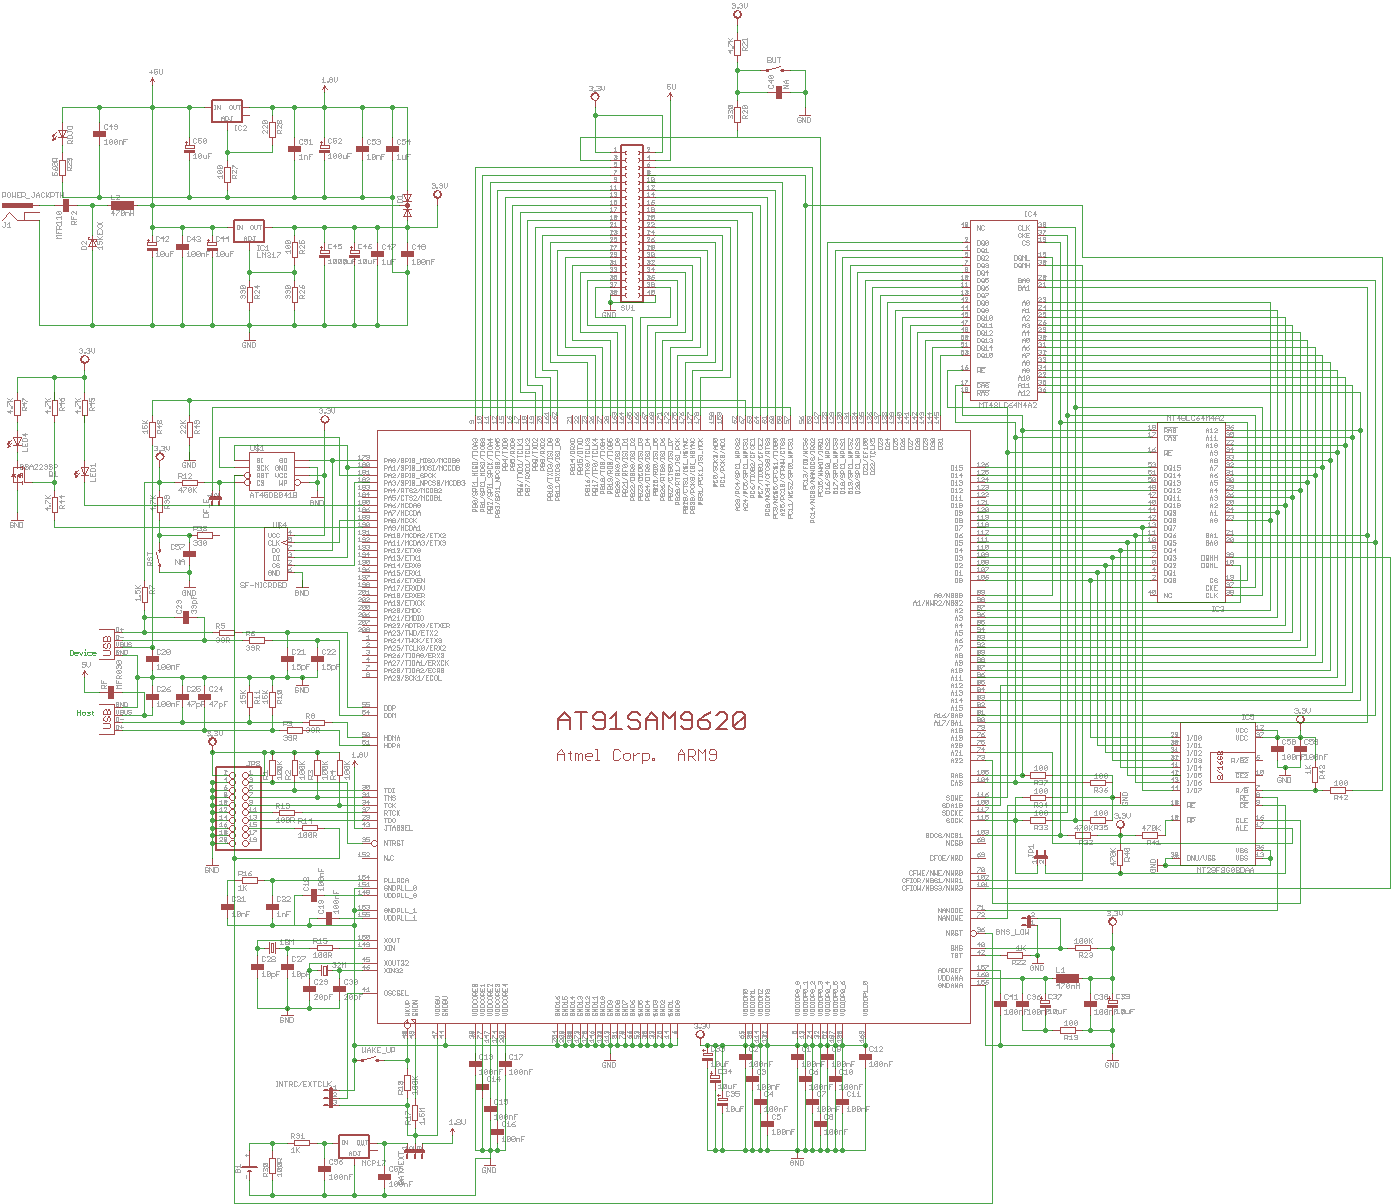
\includegraphics[scale=0.35]{appendix/samEsquematico}

\pagebreak{}

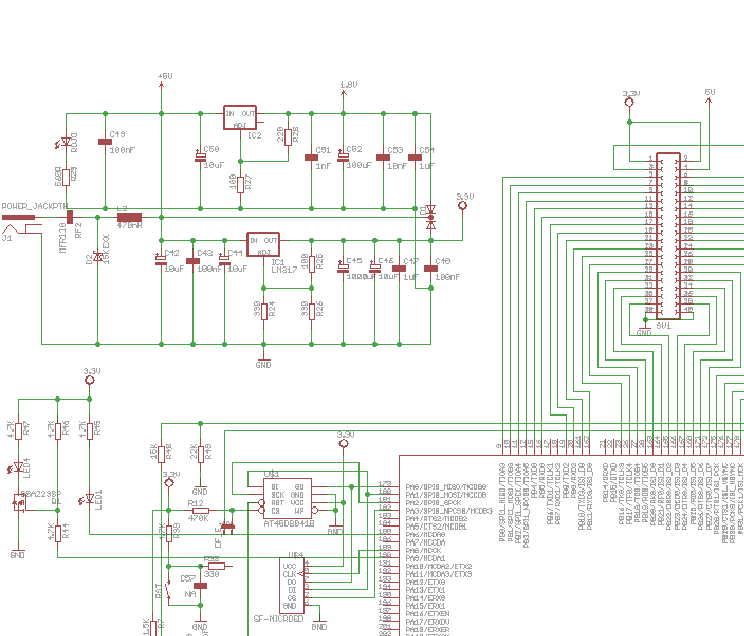
\includegraphics[scale=0.45]{appendix/samEsq1}

\ 

Parte 1 de 4. Aquí se muestran el encedido de la tarjeta, la memoria
FLASH, la tarjeta SD Card, los puertos externos, y parte del microcontrolador.

\pagebreak{}

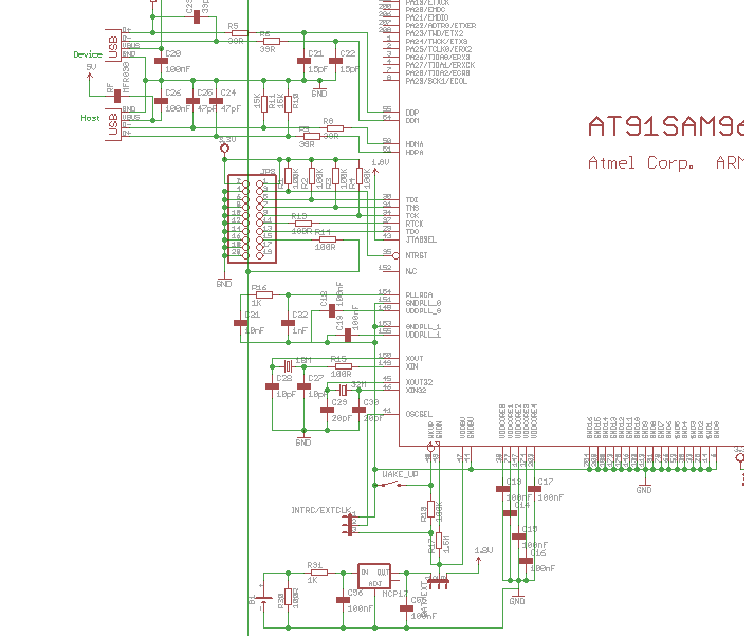
\includegraphics[scale=0.45]{appendix/samEsq2}

\ 

Parte 2 de 4. Se muestran los puertos USB y el jtag, así mismo parte
del microcontrolador.

\pagebreak{}

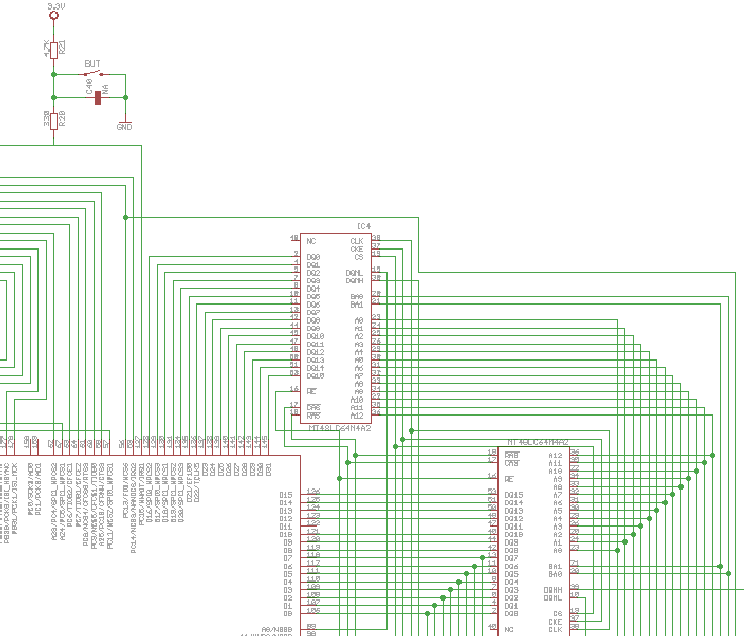
\includegraphics[scale=0.45]{appendix/samEsq3}

\ 

Parte 3 de 4. Se muestran las memorias RAM y como estan conectadas
al microcontrolador.

\pagebreak{}

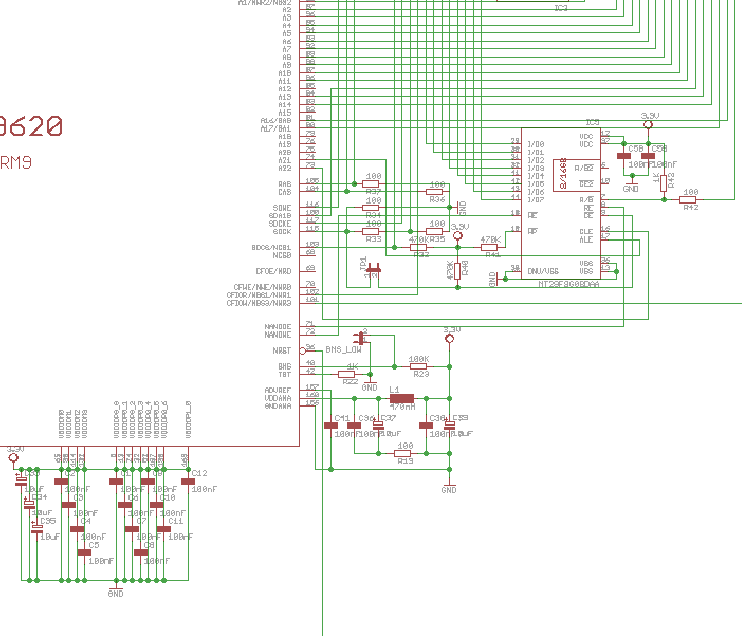
\includegraphics[scale=0.45]{appendix/samEsq4}

\ 

Parte 4 de 4. Se muestra la memoria NAND y sus conexiones con el microcontrolador
y las memorias RAM.

\pagebreak{}

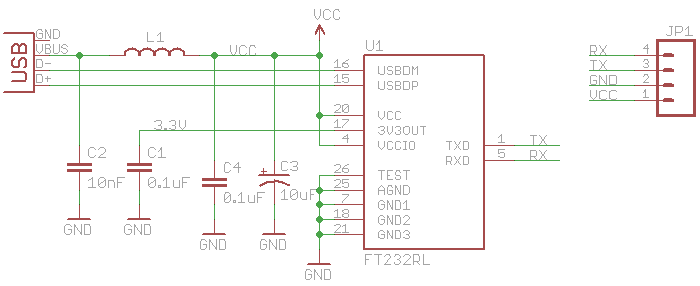
\includegraphics[scale=0.8]{appendix/ftdiEsquematico}

Diagrama del FTDI
